\let\negmedspace\undefined
\let\negthickspace\undefined
%\RequirePackage{amsmath}
\documentclass[journal,12pt,onecolumn]{IEEEtran}
 \usepackage[utf8]{inputenc}
 \usepackage{graphicx}
 \usepackage{amsmath}
 \usepackage{mathrsfs}
\usepackage{txfonts}
\usepackage{stfloats}
\usepackage{bm}
\usepackage{cite}
\usepackage{cases}
\usepackage{subfig}
 \usepackage{amsfonts}
 \usepackage{amssymb}
 \usepackage{enumitem}
\usepackage{mathtools}
\usepackage{tikz}
\usepackage{circuitikz}
\usepackage{verbatim}
\usepackage[breaklinks=false,hidelinks]{hyperref}
\usepackage{listings}
\usepackage{calc}
\usepackage{float}
\usepackage{longtable}
\usepackage{multirow}
\usepackage{multicol}
\usepackage{color}
\usepackage{array}
\usepackage{hhline}
\usepackage{ifthen}
\usepackage{chngcntr}
\usepackage{url}
\def\UrlBreaks{\do\/\do-}

\lstset{frame=single,breaklines=true,columns=fullflexible,escapechar=!@}

\newcommand{\BEQA}{\begin{eqnarray}}
\newcommand{\EEQA}{\end{eqnarray}}
\newcommand{\define}{\stackrel{\triangle}{=}}
\bibliographystyle{IEEEtran}
%\bibliographystyle{ieeetr}
\def\inputGnumericTable{}
\DeclareMathOperator*{\Res}{Res}
\let\vec\mathbf
\numberwithin{equation}{section}
\renewcommand\thesection{\arabic{section}}
\renewcommand\thesubsection{\thesection.\arabic{subsection}}
\renewcommand\thesubsubsection{\thesubsection.\arabic{subsubsection}}

\renewcommand\thesectiondis{\arabic{section}}
\renewcommand\thesubsectiondis{\thesectiondis.\arabic{subsection}}
\renewcommand\thesubsubsectiondis{\thesubsectiondis.\arabic{subsubsection}}

\providecommand{\mbf}{\mathbf}
\providecommand{\pr}[1]{\ensuremath{\Pr\left(#1\right)}}
\providecommand{\qfunc}[1]{\ensuremath{Q\left(#1\right)}}
\providecommand{\sbrak}[1]{\ensuremath{{}\left[#1\right]}}
\providecommand{\lsbrak}[1]{\ensuremath{{}\left[#1\right.}}
\providecommand{\rsbrak}[1]{\ensuremath{{}\left.#1\right]}}
\providecommand{\brak}[1]{\ensuremath{\left(#1\right)}}
\providecommand{\lbrak}[1]{\ensuremath{\left(#1\right.}}
\providecommand{\rbrak}[1]{\ensuremath{\left.#1\right)}}
\providecommand{\cbrak}[1]{\ensuremath{\left\{#1\right\}}}
\providecommand{\lcbrak}[1]{\ensuremath{\left\{#1\right.}}
\providecommand{\rcbrak}[1]{\ensuremath{\left.#1\right\}}}
\providecommand{\abs}[1]{\left\vert#1\right\vert}
\providecommand{\res}[1]{\Res\displaylimits_{#1}}
\newcommand{\myvec}[1]{\ensuremath{\begin{pmatrix}#1\end{pmatrix}}}
\newcommand{\mydet}[1]{\ensuremath{\begin{vmatrix}#1\end{vmatrix}}}
\providecommand{\gauss}[2]{\mathcal{N}\ensuremath{\left(#1,#2\right)}}
\providecommand{\gitlink}[2]{{\color{blue}\href{https://github.com/SterbenVD/AI1110-Assignments/blob/main/Assignment\%20-\%20Random\%20Numbers/#1}{#2}}}
\newcommand{\solution}{\noindent \textbf{Solution: }}
\title{Assignment: Random Numbers}
\author{Vishal Vijay Devadiga (CS21BTECH11061)}
\date{}
\begin{document}
% make the title area
\maketitle

\section{Uniform Random Numbers}
Let $U$ be a uniform random variable between 0 and 1.
\begin{enumerate}[label=\thesection.\arabic*,ref=\thesection.\theenumi]
    \item Generate $10^6$ samples of $U$ using a C program and save into a file called uni.dat.
          \\
          \solution Download the following file and execute the \gitlink{codes/1-1.c}{C program} or type in terminal:
          \begin{lstlisting}
wget https://github.com/SterbenVD/AI1110-Assignments/blob/main/Assignment\%20-\%20Random\%20Numbers/codes/1-1.c
            \end{lstlisting}
    \item
          Load the uni.dat file into python and plot the empirical CDF of $U$ using the samples in uni.dat.
          The CDF is defined as:
          \begin{align}
              F_{U}(x) = \pr{U \le x}
          \end{align}
          \begin{figure}[H]
              \centering
              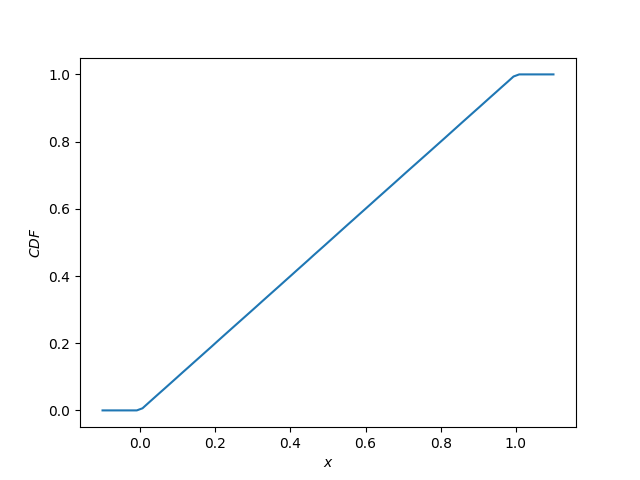
\includegraphics[scale = 0.7]{../figs/1_cdf.png}
              \caption{The CDF of $U$}
              \label{fig:1_cdf}
          \end{figure}
          \solution  The following \gitlink{codes/1-2.py}{python code} plots Fig. \ref{fig:1_cdf} or type in terminal:
          \begin{lstlisting}
wget https://github.com/SterbenVD/AI1110-Assignments/blob/main/Assignment\%20-\%20Random\%20Numbers/codes/1-2.py
            \end{lstlisting}
    \item Find a  theoretical expression for $F_{U}(x)$.
          \\
          \solution
          \begin{align}
              \label{eq:U(x)}
              U(x) =
              \begin{cases}
                  0, & x \in (-\infty,0)
                  \\
                  1, & x \in (0,1)
                  \\
                  0, & x \in (1, \infty)
              \end{cases}
          \end{align}
          By \eqref{eq:U(x)}:
          \begin{align}
                       & F_U(x) = \int_0^x U(x) dx
              \\
              \implies & F_U(x) =
              \begin{cases}
                  0, & x \in (-\infty,0)
                  \\
                  x, & x \in (0,1)
                  \\
                  1, & x \in (1, \infty)
              \end{cases}
          \end{align}
          \\
    \item
          The mean of $U$ is defined as:
          \begin{equation}
              E\sbrak{U} = \dfrac{1}{N}\sum_{i=1}^{N}U_i
          \end{equation}
          and its variance as:
          \begin{equation}
              \text{var}\sbrak{U} = E\sbrak{U- E\sbrak{U}}^2
          \end{equation}
          Write a C program to  find the mean and variance of $U$.
          \\
          \solution Download the following files and execute the \gitlink{codes/1-4.c}{C program} or type in terminal:
          \begin{lstlisting}
wget https://github.com/SterbenVD/AI1110-Assignments/blob/main/Assignment\%20-\%20Random\%20Numbers/codes/1-4.c
            \end{lstlisting}
          Values Obtained:
          \begin{align}
               & \fbox{Mean =  0.500007}
               & \fbox{Variance = 0.083301}
          \end{align}
    \item Verify your result theoretically given that:
          \begin{equation}
              E\sbrak{U^k} = \int_{-\infty}^{\infty}x^kdF_{U}(x)
          \end{equation}
          \solution
          \begin{align}
                       & dF_U(x) = p_U(x) dx
              \\
              \label{eq:U^k}
              \implies & E[U^k] = \int_{-\infty}^{\infty}x^k p_U(x) dx
          \end{align}
          Also, by \eqref{eq:U(x)}
          \begin{align}
              p_U(x) =
              \begin{cases}
                  0, & x \in (-\infty,0)
                  \\
                  1, & x \in (0,1)
                  \\
                  0, & x \in (1, \infty)
              \end{cases}
          \end{align}
          Therefore, from Equations \ref{eq:U(x)} and \ref{eq:U^k}, we have:
          \begin{align}
              E[U] & =  \int_{-\infty}^{\infty}x p_U(x) dx
              \\
                   & = \int_0 ^1 x dx
              \\
                   & = \dfrac{1}{2}
          \end{align}
          \begin{align}
              E[U^2] & =  \int_{-\infty}^{\infty}x^2 p_U(x) dx
              \\
                     & = \int_0 ^1 x^2 dx
              \\
                     & = \dfrac{1}{3}
          \end{align}
          \begin{align}
              E[U^2] - E[U]^2 & = \dfrac{1}{3} - \brak{\dfrac{1}{2}}^2
              \\
                              & = \dfrac{1}{12}
          \end{align}
          Therefore, the theoretical mean is $\dfrac{1}{2}$, and the theoretical variance is $\dfrac{1}{12}$ which closely matches the experimental values.
\end{enumerate}

\section{Central Limit Theorem}
\begin{enumerate}[label=\thesection.\arabic*,ref=\thesection.\theenumi]
    \item Generate $10^6$ samples of the random variable:
          \begin{equation}
              X = \sum_{i=1}^{12}U_i -6
          \end{equation}
          using a C program, where $U_i, i = 1,2,\dots, 12$ are  a set of independent uniform random variables between 0 and 1
          and save in a file called gau.dat.
          \\
          \solution Download the following files and execute the \gitlink{codes/2-1.c}{C program} or type in terminal:
          \begin{lstlisting}
wget https://github.com/SterbenVD/AI1110-Assignments/blob/main/Assignment\%20-\%20Random\%20Numbers/codes/2-1.c
            \end{lstlisting}
    \item Load gau.dat in python and plot the empirical CDF of $X$ using the samples in gau.dat.
          \begin{figure}[H]
              \centering
              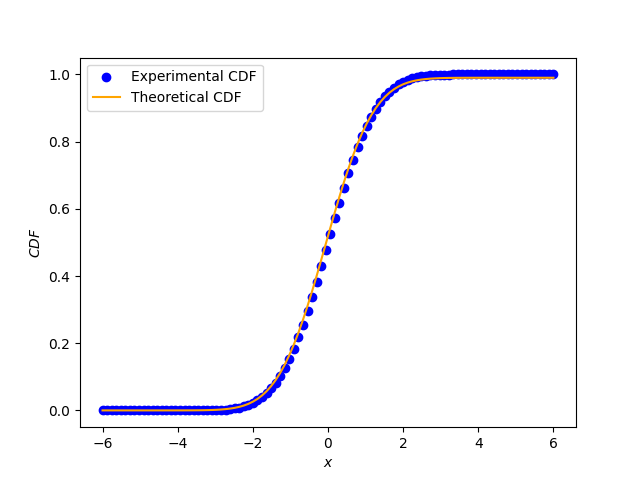
\includegraphics[scale = 0.7]{../figs/2_cdf}
              \caption{The CDF of $X$}
              \label{fig:2_cdf}
          \end{figure}
          \solution The following \gitlink{codes/2-2.py}{python code} plots Fig. \ref{fig:2_cdf}  or type in terminal:
          \begin{lstlisting}
wget https://github.com/SterbenVD/AI1110-Assignments/blob/main/Assignment\%20-\%20Random\%20Numbers/codes/2-2.py
            \end{lstlisting}
    \item Load gau.dat in python and plot the empirical PDF of $X$ using the samples in gau.dat.
          The PDF of $X$ is defined as:
          \begin{align}
              p_{X}(x) = \dfrac{d}{dx}F_{X}(x)
          \end{align}
          \begin{figure}[H]
              \centering
              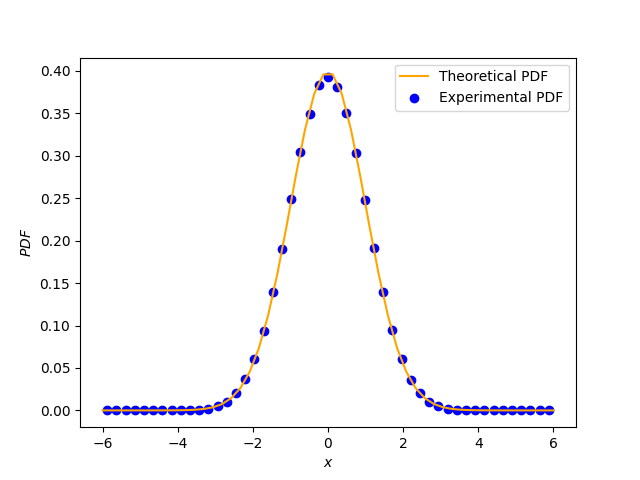
\includegraphics[scale = 0.7]{../figs/2_pdf}
              \caption{The PDF of $X$}
              \label{fig:2_pdf}
          \end{figure}
          \solution The following \gitlink{codes/2-3.py}{python code} plots Fig. \ref{fig:2_pdf} or type in terminal:
          \begin{lstlisting}
wget https://github.com/SterbenVD/AI1110-Assignments/blob/main/Assignment\%20-\%20Random\%20Numbers/codes/2-3.py
            \end{lstlisting}
    \item Find the mean and variance of $X$ by writing a C program.
          \\
          \solution Download the following files and execute the \gitlink{codes/2-4.c}{C program} or type in terminal:
          \begin{lstlisting}
wget https://github.com/SterbenVD/AI1110-Assignments/blob/main/Assignment\%20-\%20Random\%20Numbers/codes/2-4.c
            \end{lstlisting}
          Values Obtained:
          \begin{align}
               & \fbox{Mean =  -0.000241}
               & \fbox{Variance = 1.000726}
          \end{align}
    \item Given that:
          \begin{align}
              p_{X}(x) = \dfrac{1}{\sqrt{2\pi}}\exp\brak{-\dfrac{x^2}{2}}, -\infty < x < \infty,
          \end{align}
          repeat the above exercise theoretically
          \\
          \solution
          \begin{align}
              E[X] & =  \int_{-\infty}^{\infty} \dfrac{x}{\sqrt{2\pi}}\exp{\left(-\dfrac{x^2}{2}\right)}
              \\
                   & = -\dfrac{1}{\sqrt{2\pi}}\exp\brak{-\dfrac{x^2}{2}} \Bigg{|}_{-\infty}^{\infty}
              \\
                   & = 0
          \end{align}
          Also,
          \begin{align}
              E[X^2] & =  \int_{-\infty}^{\infty} \dfrac{x^2}{\sqrt{2\pi}}\exp{\left(-\dfrac{x^2}{2}\right)}
              \\
                     & = -\dfrac{x}{\sqrt{2\pi}}e^{\brak{-\dfrac{x^2}{2}}} \Bigg{|}_{-\infty}^{\infty} + \int_{-\infty}^{\infty} \dfrac{1}{\sqrt{2\pi}}e^{\brak{-\dfrac{x^2}{2}}}
              \\
                     & = 0 + \dfrac{1}{\sqrt{2\pi}} \times \sqrt{2\pi}
              \\
                     & = 1
          \end{align}
          Thus,
          \begin{align}
              \text{var}(X) & = E[X^2] - E[X]^2 \\
                            & = 1
          \end{align}
          Therefore, the mean is $0$ and the variance is $1$.
\end{enumerate}

\section{From Uniform to Other}
\begin{enumerate}[label=\thesection.\arabic*,ref=\thesection.\theenumi]
    \item
          Generate samples of:
          \begin{equation}
              V = -2\ln\brak{1-U}
          \end{equation}
          and plot its CDF.
          \\
          \solution
          \begin{figure}[H]
              \centering
              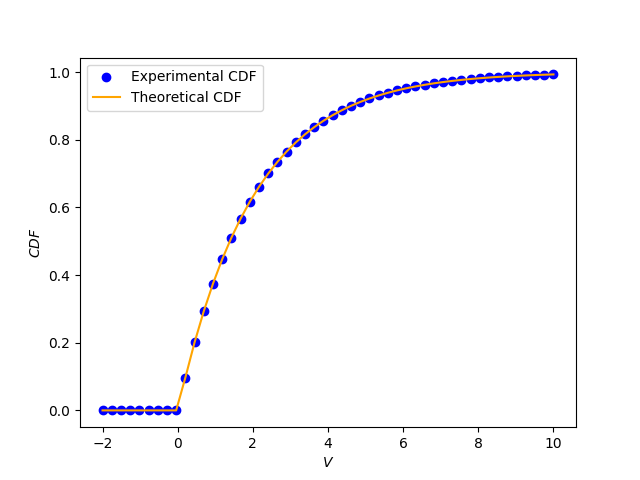
\includegraphics[scale = 0.6]{../figs/3_cdf}
              \caption{The CDF of $V$}
              \label{fig:3_cdf}
          \end{figure}
          The following \gitlink{codes/3-1.py}{python code} plots Fig. \ref{fig:3_cdf} or type in terminal:
          \begin{lstlisting}
wget https://github.com/SterbenVD/AI1110-Assignments/blob/main/Assignment\%20-\%20Random\%20Numbers/codes/3-1.py
            \end{lstlisting}
    \item Find a theoretical expression for $F_V(x)$.
          \\
          \solution
          \begin{align}
              F_V(x) & = \pr{V \leq x}
              \\
                     & = \pr{-2\ln(1-U) \leq x}
              \\
                     & = \pr{1-U \geq	\exp{\left(-\dfrac{x}{2}\right)}}
              \\
                     & = \pr{U \leq 1 - \exp{\left(-\dfrac{x}{2}\right)}}
              \\
                     & = F_U\left(1 - \exp{\left(-\dfrac{x}{2}\right)}\right)
          \end{align}
          Therefore,
          \begin{align}
                       & F_V(x) =
              \begin{cases}
                  0,                                    & 1 - \exp{\left(-\dfrac{x}{2}\right)} \in (-\infty,0)
                  \\
                  1 - \exp{\left(-\dfrac{x}{2}\right)}, & 1 - \exp{\left(-\dfrac{x}{2}\right)} \in (0,1)
                  \\
                  1,                                    & 1 - \exp{\left(-\dfrac{x}{2}\right)} \in (1, \infty)
              \end{cases}
              \\
              \implies & F_V(x) =
              \begin{cases}
                  0,                                    & x \in (-\infty,0)
                  \\
                  1 - \exp{\left(-\dfrac{x}{2}\right)}, & x \in (0,\infty)
              \end{cases}
          \end{align}
\end{enumerate}

\section{Triangular Distribution}
\begin{enumerate}[label=\thesection.\arabic*
        ,ref=\thesection.\theenumi]
    %
    \item Generate
          \begin{align}
              T = U_1+U_2
          \end{align}
          \solution Download the following files and execute the \gitlink{codes/4-1.c}{C program} or type in terminal:
          \begin{lstlisting}
wget https://github.com/SterbenVD/AI1110-Assignments/blob/main/Assignment\%20-\%20Random\%20Numbers/codes/4-1.c
            \end{lstlisting}
    \item Find the CDF of $T$.
          \\
          \solution
          \begin{figure}[H]
              \centering
              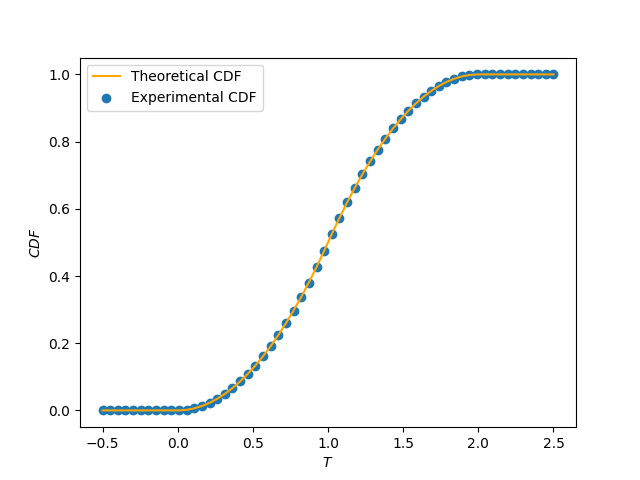
\includegraphics[scale = 0.5]{../figs/4_cdf}
              \caption{The CDF of $V$}
              \label{fig:4_cdf}
          \end{figure}
          The following \gitlink{codes/4-2.py}{python code} plots Fig. \ref{fig:4_cdf} or type in terminal:
          \begin{lstlisting}
wget https://github.com/SterbenVD/AI1110-Assignments/blob/main/Assignment\%20-\%20Random\%20Numbers/codes/4-2.py
            \end{lstlisting}
    \item Find the PDF of $T$.
          \\
          \solution\begin{figure}[H]
              \centering
              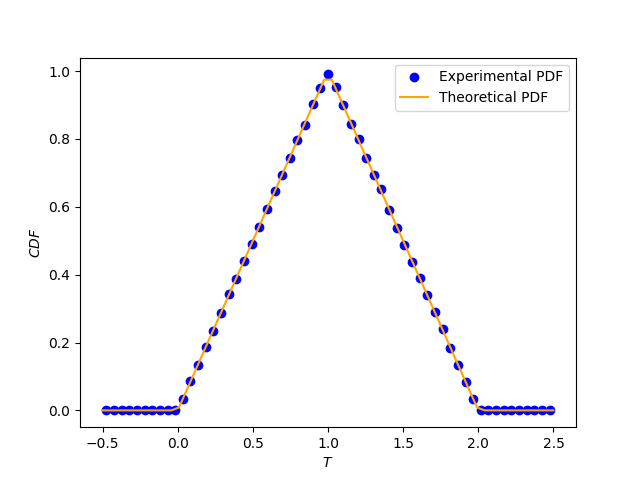
\includegraphics[scale = 0.9]{../figs/4_pdf}
              \caption{The PDF of $T$}
              \label{fig:4_pdf}
          \end{figure}
          \solution The following \gitlink{codes/4-3.py}{python code} plots Fig. \ref{fig:4_pdf} or type in terminal:
          \begin{lstlisting}
wget https://github.com/SterbenVD/AI1110-Assignments/blob/main/Assignment\%20-\%20Random\%20Numbers/codes/4-3.py
      \end{lstlisting}
    \item Find the theoretical expressions for the PDF and CDF of $T$. \\
          \solution
          \begin{align}
              T = U_1 + U_2
          \end{align}
          Thus we have:
          \begin{align}
              p_T(t) & = (p_{U_1} * p_{U_2})(t)
              \\
                     & = \int _{-\infty} ^{\infty} p_U(u) p_U(t-u) du
              \\
                     & = \int _0 ^1 p_U(t-u) du
          \end{align}
          When $0 < t < 1$:
          \begin{align}
              p_T(t) & = \int _0 ^1 p_U(t-u) du
              \\
                     & = \int _0 ^t p_U(t-u) du
              \\
                     & = \int _0 ^t du
              \\
                     & = t
          \end{align}
          when $ 1 < t < 2$:
          \begin{align}
              p_T(t) & = \int _0 ^1 p_U(t-u) du
              \\
                     & = \int _{t-1} ^1 p_U(t-u) du
              \\
                     & = \int _{t-1} ^1 du
              \\
                     & = 2-t
          \end{align}
          When $t < 0$ and $t > 2$ , the integral evaluates to $0$. Thus,
          \begin{align}
              p_T(t) =
              \begin{cases}
                  0,   & t \in (-\infty,0)
                  \\
                  t,   & t \in (0,1)
                  \\
                  2-t, & t \in (1, 2)
                  \\
                  0,   & t \in (2,\infty)
              \end{cases}
          \end{align}
          For CDF of T:
          \begin{align}
                       & F_T(t) = \int _{-\infty} ^t p_T(x) dx
              \\
              \implies & F_T(t) =
              \begin{cases}
                  0,                       & t \in (-\infty,0)
                  \\
                  \frac{t^2}{2},           & t \in (0,1)
                  \\
                  -\frac{t^2}{2} + 2t - 1, & t \in (1, 2)
                  \\
                  1,                       & t \in (2,\infty)
              \end{cases}
          \end{align}
    \item Verify your results through a plot. \\
          \solution Fig.\ref{fig:4_cdf} and Fig.\ref{fig:4_pdf} plots the theoretical cdf and pdf respectively, which closely matches the experimental values.
\end{enumerate}
\section{Maximul Likelihood}
\begin{enumerate}[label=\thesection.\arabic*
        ,ref=\thesection.\theenumi]
    \item Generate
          \begin{equation}
              Y = AX+N,
          \end{equation}
          where $A = 5 \text{ dB}, X$ \i $\cbrak{1,-1}$,  is Bernoulli and $N \sim \gauss{0}{1}$.
    \item Plot $Y$.
    \item Guess how to estimate $X$ from $Y$.
    \item
          \label{ml-ch4_sim}
          Find
          \begin{equation}
              P_{e|0} = \pr{\hat{X} = -1|X=1}
          \end{equation}
          and
          \begin{equation}
              P_{e|1} = \pr{\hat{X} = 1|X=-1}
          \end{equation}
          %
    \item Find $P_e$.
          %
    \item
          Verify by plotting  the theoretical $P_e$.
\end{enumerate}
\section{Gaussian to Other}
\begin{enumerate}[label=\thesection.\arabic*
        ,ref=\thesection.\theenumi]
    \item
          Let $X_1 \sim  \gauss{0}{1}$ and $X_2 \sim  \gauss{0}{1}$. Plot the CDF and PDF of
          %
          \begin{equation}
              V = X_1^2 + X_2^2
          \end{equation}
          %
          %
          %
    \item
          If
          %
          \begin{equation}
              F_{V}(x) =
              \begin{cases}
                  1 - e^{-\alpha x} & x \geq 0 \\
                  0                 & x < 0,
              \end{cases}
          \end{equation}
          %
          find $\alpha$.
          %
    \item
          \label{ch3_raleigh_sim}
          Plot the CDF and PDf of
          %
          \begin{equation}
              A = \sqrt{V}
          \end{equation}
          %
\end{enumerate}
\section{Conditional Probability}
\begin{enumerate}[label=\thesection.\arabic*
        ,ref=\thesection.\theenumi]
    \item
    \item
          \label{ch4_sim}
          Plot
          \begin{equation}
              P_e = \pr{\hat{X} = -1|X=1}
          \end{equation}
          %
          for
          \begin{equation}
              Y = AX+N,
          \end{equation}
          where $A$ is Raleigh with $E\sbrak{A^2} = \gamma, N \sim \gauss{0}{1}, X \in \brak{-1,1}$ for $0 \le \gamma \le 10$ dB.
          %
    \item
          Assuming that $N$ is a constant, find an expression for $P_e$.  Call this $P_e(N)$
          %
    \item
          %
          \label{ch4_anal}
          For a function $g$,
          \begin{equation}
              E\sbrak{g(X)} = \int_{-\infty}^{\infty}g(x)p_{X}(x)\, dx
          \end{equation}
          %
          Find $P_e = E\sbrak{P_e(N)}$.
          %
    \item
          Plot $P_e$ in problems \ref{ch4_sim} and \ref{ch4_anal} on the same graph w.r.t $\gamma$.  Comment.
\end{enumerate}
\section{Two Dimensions}
Let
\begin{equation}
    \mbf{y} = A\mbf{x} + \mbf{n},
\end{equation}
where
\begin{align}
    x       & \in \brak{\mbf{s}_0,\mbf{s}_1},
    \mbf{s}_0 =
    \begin{pmatrix}
        1
        \\
        0
    \end{pmatrix},
    \mbf{s}_1 =
    \begin{pmatrix}
        0
        \\
        1
    \end{pmatrix}
    \\
    \mbf{n} & =
    \begin{pmatrix}
        n_1
        \\
        n_2
    \end{pmatrix},
    n_1,n_2 \sim \gauss{0}{1}.
\end{align}
%
\begin{enumerate}[label=\thesection.\arabic*
        ,ref=\thesection.\theenumi]
    %%
    \item
          \label{ch5_fsk}
          Plot
          %
          \begin{equation}
              \mbf{y}|\mbf{s}_0 \text{ and } \mbf{y}|\mbf{s}_1
          \end{equation}
          %
          on the same graph using a scatter plot.
          %
    \item
          For the above problem, find a decision rule for detecting the symbols $\mbf{s}_0 $ and $\mbf{s}_1$.
          %
    \item
          Plot
          \begin{equation}
              P_e = \pr{\hat{\mbf{x}} = \mbf{s}_1|\mbf{x} = \mbf{s}_0}
          \end{equation}
          with respect to the SNR from 0 to 10 dB.
          %
    \item
          Obtain an expression for $P_e$. Verify this by comparing the theory and simulation plots on the same graph.
          %
\end{enumerate}
\end{document}
